\documentclass[tikz,border=8pt]{standalone}
% Shared look for every TikZ diagram. Load with \input{../../tools/tikz-style.tex}
\usepackage[sfdefault]{roboto}
\usetikzlibrary{arrows.meta, positioning, shapes.geometric, calc, fit, backgrounds}
\definecolor{cblue}{HTML}{4C78A8}
\definecolor{corange}{HTML}{F58518}
\definecolor{cgreen}{HTML}{54A24B}
\definecolor{cred}{HTML}{E45756}
\definecolor{cpurple}{HTML}{B279A2}
\definecolor{cgrey}{HTML}{6B6B6B}
\tikzset{
  every picture/.style={font=\sffamily, line width=1.2pt},
  box/.style={draw=#1, fill=#1!12, rounded corners=4pt, align=center, inner sep=7pt, minimum height=1.1cm},
  box/.default=cgrey,
  arrow/.style={-{Stealth[length=3mm]}, draw=cgrey, line width=1.4pt},
  title/.style={font=\sffamily\bfseries\Large},
  note/.style={font=\sffamily\small, text=cgrey, align=center},
}
\AtBeginDocument{\hyphenpenalty=10000 \exhyphenpenalty=10000}

% The speed loop as a computer runs it (FBS Fig. 8.14; CTM digital tutorial): a clock ticks every T = 0.01 s; at each
% tick the A/D reads the speed, the computer runs the PI's difference equation, and the D/A sends out the force, which
% the zero-order hold keeps constant until the next tick. Small sketches show the kind of signal on each wire:
% smooth (continuous), dots (samples, numbers) or a staircase (held numbers).
\begin{document}
\begin{tikzpicture}[every node/.append style={font=\large}]
  \node[box=cblue, text width=6.2cm] (comp) at (0,0) {\textbf{computer}, once per tick\\[4pt]
     $e_k = r - v_k$\\[2pt] $u_k = 20\,e_k + I_k$\\[2pt] $I_{k+1} = I_k + 10\,T\,e_k$};
  \node[box=corange, text width=4.6cm] (da) at (9.4,0) {\textbf{D/A converter}\\ and \textbf{zero-order hold}\\[3pt]
     \small holds $u_k$ for $T$};
  \node[box=cgrey, text width=4.6cm] (robot) at (9.4,-6.0) {\textbf{motors and robot}\\[3pt]
     $8\,\dfrac{dv}{dt} = u - 2\,v$};
  \node[box=cgreen, text width=4.6cm] (ad) at (0,-6.0) {\textbf{A/D converter}\\[3pt]
     \small reads the speed $v$\\ at $t = kT$};
  \node[box=cpurple, text width=3.6cm] (clock) at (4.7,-3.0) {\textbf{clock}\\[2pt] \small a tick every\\ $T = 0.01$ s};
  % reference in
  \draw[arrow] (-4.8,0) -- node[above] {$r$} node[below, font=\small, text=cgrey] {0.5 m/s} (comp.west);
  % computer -> D/A: numbers
  \draw[arrow] (comp.east) -- node[above] {$u_k$ (numbers)} (da.west);
  \foreach \i/\h in {0/0.25,1/0.45,2/0.35} {\fill[cblue] (4.15+0.45*\i,-0.42+\h*0.6) circle (2.2pt);}
  % D/A -> robot: staircase
  \draw[arrow] (da.south) -- node[right, align=left] {force $u(t)$\\ \small a staircase} (robot.north);
  \draw[corange, line width=1.2pt] (7.5,-2.4) -- ++(0.35,0) -- ++(0,0.3) -- ++(0.35,0) -- ++(0,-0.15) -- ++(0.35,0)
     -- ++(0,0.2) -- ++(0.35,0);
  % robot -> A/D: smooth speed
  \draw[arrow] (robot.west) -- node[below] {speed $v(t)$, smooth} (ad.east);
  \draw[cgrey, line width=1.2pt] (3.6,-5.45) .. controls (4.3,-5.0) and (5.0,-5.1) .. (5.8,-5.2);
  % A/D -> computer: samples
  \draw[arrow] (ad.north) -- node[left, align=right] {$v_k$ (numbers)\\ \small one per tick} (comp.south);
  \foreach \i/\h in {0/0.1,1/0.45,2/0.6} {\fill[cgreen] (0.45+0.38*\i,-3.6+\h*0.6) circle (2.2pt);}
  % the clock drives the A/D and the D/A
  \draw[cpurple, dashed, line width=1.2pt, -{Stealth[length=2.5mm]}] (clock.north east) -- (da.south west);
  \draw[cpurple, dashed, line width=1.2pt, -{Stealth[length=2.5mm]}] (clock.south west) -- (ad.north east);
\end{tikzpicture}
\end{document}
